\documentclass[12pt,a4paper]{report}

% ─── Packages ────────────────────────────────────────────────────────────────
\usepackage[T1]{fontenc}
\usepackage[utf8]{inputenc}
\usepackage[a4paper, margin=2.5cm]{geometry}
\usepackage{graphicx}
\usepackage{booktabs}
\usepackage{longtable}
\usepackage{array}
\usepackage{tabularx}
\usepackage{xcolor}
\usepackage{listings}
\usepackage{hyperref}
\usepackage{fancyhdr}
\usepackage{titlesec}
\usepackage{setspace}
\usepackage{caption}
\usepackage{subcaption}
\usepackage{amsmath}
\usepackage{float}
\usepackage{parskip}
\usepackage{enumitem}
\usepackage{pdfpages}

% ─── Colours ─────────────────────────────────────────────────────────────────
\definecolor{codebg}{RGB}{248,248,248}
\definecolor{codeframe}{RGB}{200,200,200}
\definecolor{keywordcolor}{RGB}{0,0,180}
\definecolor{commentcolor}{RGB}{60,120,60}
\definecolor{stringcolor}{RGB}{160,0,0}
\definecolor{headingblue}{RGB}{31,73,125}

% ─── Hyperref ────────────────────────────────────────────────────────────────
\hypersetup{
    colorlinks=true,
    linkcolor=headingblue,
    urlcolor=headingblue,
    citecolor=headingblue,
    pdftitle={Design and Implementation of a Parallel-In Serial-Out (PISO) Shift Register on FPGA},
    pdfauthor={Molik Rajvanshi, Shivam Tiwari, Ujjawal Khatri},
}

% ─── Listings (code) ─────────────────────────────────────────────────────────
\lstdefinelanguage{VHDL}{
    morekeywords={library, use, entity, is, generic, port, in, out,
                  STD_LOGIC, STD_LOGIC_VECTOR, INTEGER, unsigned,
                  architecture, of, signal, begin, end, process,
                  if, then, elsif, else, rising_edge, downto, others,
                  when, wait, constant, component, map, port, generic,
                  not, and, or, xor, to, range},
    keywordstyle=\color{keywordcolor}\bfseries,
    comment=[l]{--},
    commentstyle=\color{commentcolor}\itshape,
    stringstyle=\color{stringcolor},
    sensitive=false,
    morestring=[b]",
}

\lstdefinelanguage{XDC}{
    keywords={set\_property, create\_clock, get\_ports},
    keywordstyle=\color{keywordcolor}\bfseries,
    comment=[l]{\#\#},
    commentstyle=\color{commentcolor}\itshape,
    sensitive=false,
}

\lstset{
    backgroundcolor=\color{codebg},
    frame=single,
    rulecolor=\color{codeframe},
    basicstyle=\ttfamily\footnotesize,
    breaklines=true,
    breakatwhitespace=false,
    keepspaces=true,
    showspaces=false,
    showstringspaces=false,
    tabsize=4,
    captionpos=b,
    numbers=left,
    numberstyle=\tiny\color{gray},
    numbersep=8pt,
    xleftmargin=15pt,
    xrightmargin=5pt,
}

% ─── Section heading styles ──────────────────────────────────────────────────
\titleformat{\chapter}[block]
  {\normalfont\Large\bfseries\color{headingblue}}
  {\thechapter.}{0.5em}{}
\titlespacing*{\chapter}{0pt}{10pt}{15pt}

\titleformat{\section}
  {\normalfont\large\bfseries\color{headingblue}}
  {\thesection}{0.5em}{}

\titleformat{\subsection}
  {\normalfont\normalsize\bfseries\color{headingblue}}
  {\thesubsection}{0.5em}{}

% ─── Header / Footer ─────────────────────────────────────────────────────────
\pagestyle{fancy}
\fancyhf{}
\fancyhead[L]{\small PISO Shift Register on FPGA}
\fancyhead[R]{\small B.Tech ECE Project}
\fancyfoot[C]{\thepage}
\renewcommand{\headrulewidth}{0.4pt}

% ─── Misc helpers ────────────────────────────────────────────────────────────
\setlength{\parskip}{6pt}
\setlength{\parindent}{0pt}
\captionsetup{font=small, labelfont=bf}

% ─────────────────────────────────────────────────────────────────────────────
\begin{document}

% ══════════════════════════════════════════════════════════════════════════════
%  TITLE PAGE
% ══════════════════════════════════════════════════════════════════════════════
\begin{titlepage}
  \centering
  \vspace*{1.5cm}

  {\LARGE\bfseries
    Design and Implementation of a\\[6pt]
    Parallel-In Serial-Out (PISO) Shift Register\\[6pt]
    on FPGA\par}

  \vspace{1.2cm}

  {\normalsize Project submitted for the fulfillment of the\par}
  \vspace{0.3cm}
  {\normalsize Requirements of the degree of\par}

  \vspace{0.8cm}

  {\normalsize Bachelor of Technology\par}
  \vspace{0.2cm}
  {\normalsize Electronics and Communication Technology\par}

  \vspace{1.2cm}

  {\normalsize
    Molik Rajvanshi- 23UEC575\\[3pt]
    Shivam Tiwari- 23UEC622\\[3pt]
    Ujjawal Khatri- 23UEC635\par}

  \vspace{0.5cm}

  {\normalsize
    Email :
    \href{mailto:23uec575@lnmiit.ac.in}{23uec575@lnmiit.ac.in}\\[2pt]
    \phantom{Email :\ }
    \href{mailto:23uec622@lnmiit.ac.in}{23uec622@lnmiit.ac.in}\\[2pt]
    \phantom{Email :\ }
    \href{mailto:23uec635@lnmiit.ac.in}{23uec635@lnmiit.ac.in}\par}

  \vspace{1.2cm}

  {\normalsize
    Project Supervisor-:\\[3pt]
    Dr. Kusum Lata\par}

  \vspace{1.0cm}

  \includegraphics[width=5cm]{images/lnmiit_logo.png}

  \vspace{0.75cm}

  {\normalsize
    Department of Electronics and Communication\\
    Engineering- The LNM Institute of Information\\
    Technology, Jaipur\par}

\end{titlepage}

% ══════════════════════════════════════════════════════════════════════════════
%  TABLE OF CONTENTS
% ══════════════════════════════════════════════════════════════════════════════
\tableofcontents
\listoffigures
\listoftables
\newpage

% ══════════════════════════════════════════════════════════════════════════════
\chapter{Objective}
% ══════════════════════════════════════════════════════════════════════════════

This project designs and implements an 8-bit Parallel-In Serial-Out (PISO) shift register on the Nexys 4 DDR FPGA development board, using VHDL as the hardware description language and Vivado 2022.1 as the design environment.

The PISO shift register accepts an 8-bit parallel data word (supplied via DIP switches SW[7:0]) and, when triggered by the centre button (\texttt{load}), serialises and transmits it MSB-first over a single output pin (\texttt{serial\_out}) at a visually observable rate of approximately 1--2\,Hz. A \texttt{busy} signal indicates when a transmission is in progress, and an active-low reset (CPU\_RESETN) clears the internal state at any time.

\textbf{Specific objectives:}
\begin{itemize}[leftmargin=1.5em]
  \item Implement a clean, synchronous PISO shift-register architecture in VHDL with a configurable \texttt{WIDTH} generic.
  \item Design a 26-bit clock divider to derive a slow ($\approx$1.5\,Hz) shift clock from the 100\,MHz system oscillator, making individual bit transmissions visible on the FPGA's LEDs.
  \item Map all I/O to physical pins on the Nexys 4 DDR using a Vivado XDC constraints file.
  \item Verify correct operation with a behavioural simulation testbench (two test patterns: \texttt{0xAB} and \texttt{0xCC}).
  \item Synthesize and implement the design, achieving timing closure and minimal resource utilisation.
\end{itemize}

% ══════════════════════════════════════════════════════════════════════════════
\chapter{Tools and Resources Used}
% ══════════════════════════════════════════════════════════════════════════════

\begin{itemize}[leftmargin=1.5em]
  \item \textbf{Development Board:} Nexys 4 DDR --- Xilinx Artix-7 XC7A100T-1CSG324C, 100\,MHz on-board oscillator.
  \item \textbf{Design Software:} Vivado 2022.1 --- for synthesis, implementation, bitstream generation, and behavioural simulation.
  \item \textbf{HDL Language:} VHDL (IEEE 1076-2008) --- used for both the synthesizable design unit (\texttt{piso.vhd}) and the testbench (\texttt{tb.vhd}).
  \item \textbf{Simulation Tool:} Vivado Simulator (xsim) --- used for functional behavioural simulation; waveforms viewed in the integrated waveform viewer.
  \item \textbf{IP Cores Used:} None --- all logic (clock divider, shift register) implemented manually for pedagogical clarity.
  \item \textbf{Physical I/O:} DIP switches SW[7:0] for parallel input, CPU\_RESETN button for active-low reset, centre button for \texttt{load} trigger, LED0 for \texttt{serial\_out}, LED1 for \texttt{busy}.
\end{itemize}

% ══════════════════════════════════════════════════════════════════════════════
\chapter{System Design / Architecture}
% ══════════════════════════════════════════════════════════════════════════════

\section{Overview}

A Parallel-In Serial-Out (PISO) shift register takes an $n$-bit parallel word and converts it to a single-bit serial stream, sending one bit per clock cycle, MSB first. This is a fundamental building block in serial communication protocols (SPI, I\textsuperscript{2}C, UART). In this implementation, the shift clock is deliberately slowed to $\approx$1.5\,Hz so that the progression of bits can be observed directly on the FPGA's LEDs with the naked eye.

\section{Architecture Block Description}

The design is contained in a single VHDL entity \texttt{parallel\_to\_serial\_selector} with the \texttt{rtl} architecture. Internally it is composed of two concurrent processes:

\textbf{Clock Divider Process} \\
A 26-bit unsigned counter (\texttt{counter}) increments on every rising edge of the 100\,MHz \texttt{clk}. The signal \texttt{slow\_clk} is driven from \texttt{counter(25)}, which toggles every $2^{25}$ cycles. This produces a \texttt{slow\_clk} full period of:
\[
  T_{\text{slow}} = 2^{26} \times 10\,\text{ns} \approx 671\,\text{ms} \quad (f \approx 1.49\,\text{Hz})
\]
This is the clock that drives the shift register, making each bit output visible for about 335\,ms.

\textbf{Main PISO Process} \\
This process is sensitive to \texttt{slow\_clk} and \texttt{reset}. The logic follows three states:
\begin{itemize}[leftmargin=1.5em]
  \item \textbf{Reset (async, active-low):} \texttt{reset = '0'} clears \texttt{shift\_reg}, \texttt{bit\_count}, \texttt{serial\_out}, and \texttt{active}.
  \item \textbf{Load:} On \texttt{rising\_edge(slow\_clk)}, if \texttt{load = '1'} and \texttt{active = '0'}, the parallel input is latched into \texttt{shift\_reg}, \texttt{bit\_count} is set to \texttt{WIDTH} (8), and \texttt{active} is asserted.
  \item \textbf{Shift:} While \texttt{active = '1'}, on each \texttt{rising\_edge(slow\_clk)}, \texttt{shift\_reg(WIDTH-1)} (the MSB) is driven onto \texttt{serial\_out}, the register is left-shifted by one and zero-filled on the right, and \texttt{bit\_count} is decremented. When \texttt{bit\_count} reaches 1, \texttt{active} is de-asserted, ending the transmission.
\end{itemize}

The \texttt{busy} output is a direct alias of \texttt{active} and stays high for the entire duration of a shift operation.

\section{Signal and Generic Summary}

\begin{table}[H]
  \centering
  \caption{Entity ports and generics of \texttt{parallel\_to\_serial\_selector}}
  \label{tab:ports}
  \begin{tabularx}{\linewidth}{llllX}
    \toprule
    \textbf{Name} & \textbf{Direction} & \textbf{Type} & \textbf{Width} & \textbf{Description} \\
    \midrule
    \texttt{WIDTH}       & Generic & \texttt{INTEGER} & ---    & Number of bits to shift (default 8) \\
    \texttt{clk}         & in      & \texttt{STD\_LOGIC} & 1   & 100\,MHz system clock \\
    \texttt{reset}       & in      & \texttt{STD\_LOGIC} & 1   & Active-low asynchronous reset \\
    \texttt{load}        & in      & \texttt{STD\_LOGIC} & 1   & Load enable (edge-sampled on slow\_clk) \\
    \texttt{parallel\_in}& in      & \texttt{STD\_LOGIC\_VECTOR} & 8 & 8-bit parallel data word \\
    \texttt{serial\_out} & out     & \texttt{STD\_LOGIC} & 1   & MSB-first serial bit stream \\
    \texttt{busy}        & out     & \texttt{STD\_LOGIC} & 1   & High while shift is in progress \\
    \bottomrule
  \end{tabularx}
\end{table}

\section{RTL Schematic}

The RTL schematic below was generated by Vivado after elaboration. It shows 53 cells, 13 I/O ports, and 104 nets. Key elements visible include the 26-bit \texttt{RTL\_ADD}/\texttt{RTL\_REG} counter chain (bottom-left), the \texttt{RTL\_SUB} bit-counter logic, the \texttt{RTL\_MUX} select trees for load vs. shift operation, the \texttt{RTL\_ROM} lookup used for the active flag, and the async-reset \texttt{RTL\_REG\_ASYNC} registers for \texttt{shift\_reg[7:0]}, \texttt{active\_reg}, and \texttt{serial\_out\_reg}.

\begin{figure}[H]
  \centering
  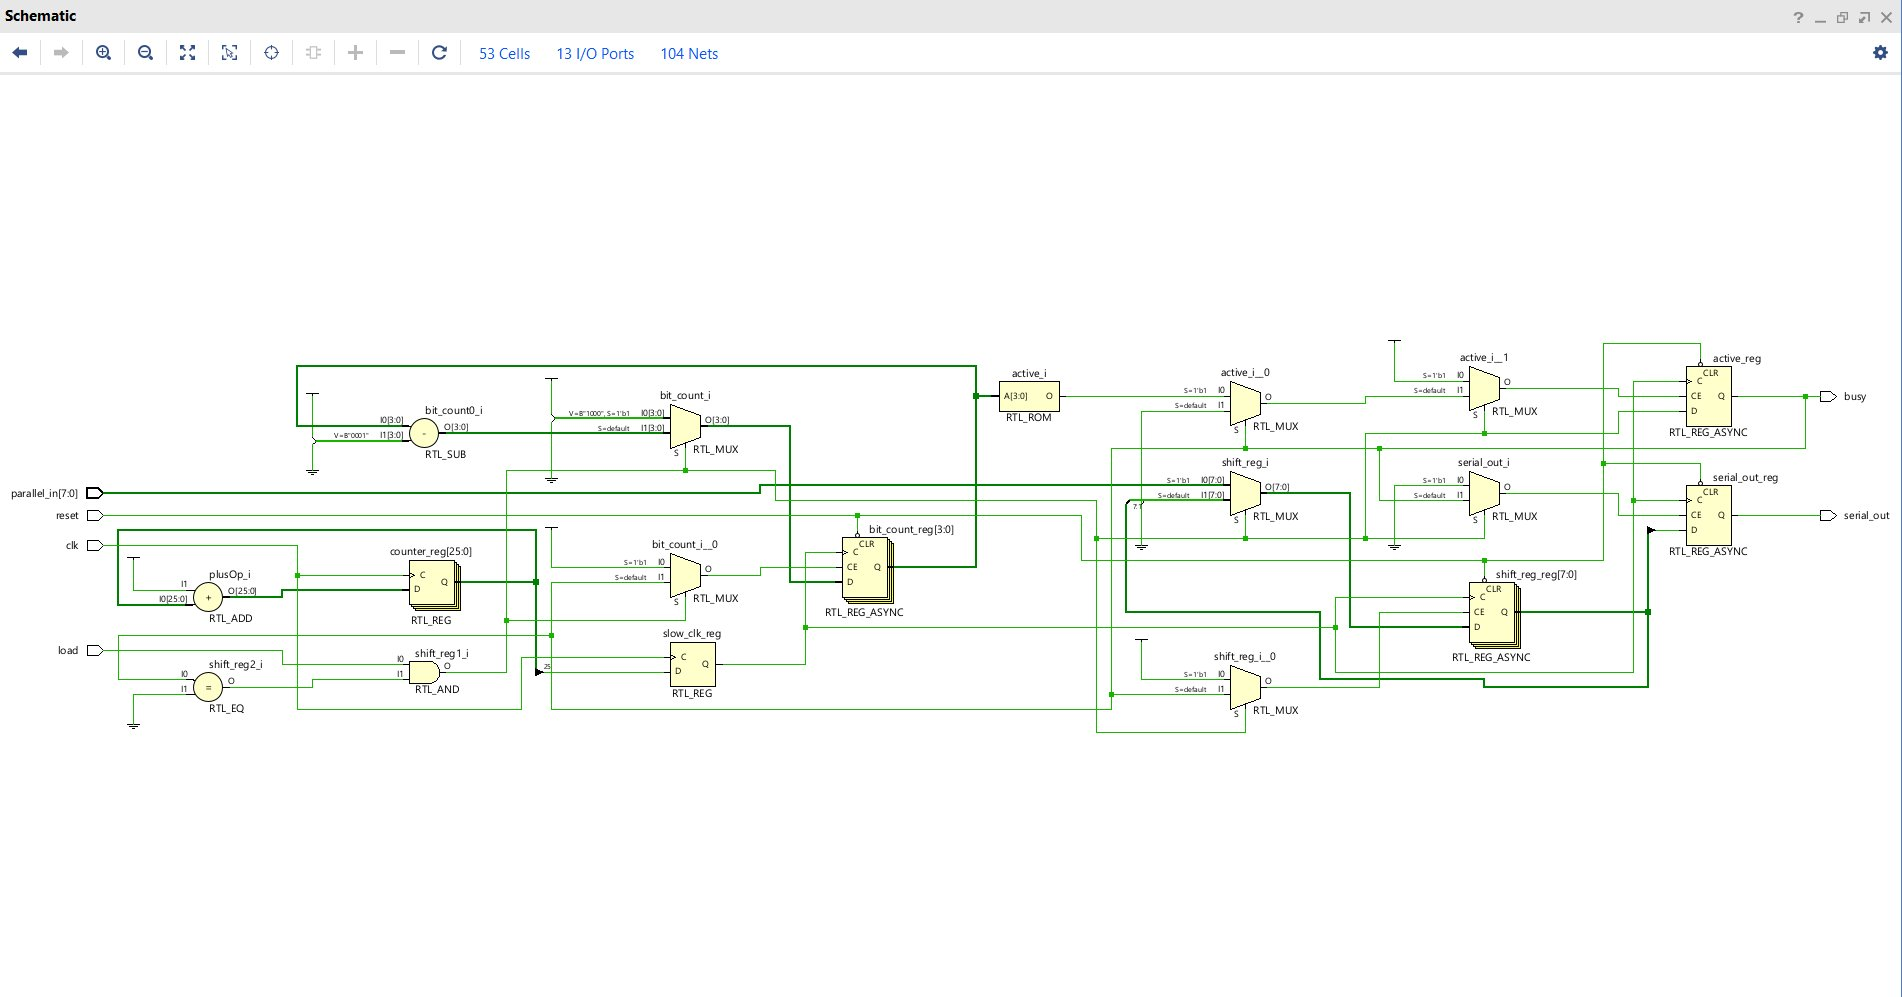
\includegraphics[width=\linewidth]{images/rtl_schematic.png}
  \caption{Vivado-generated RTL schematic of the PISO shift register (53 cells, 13 I/O ports, 104 nets): clock divider counter chain (bottom-left), bit-count subtractor, load/shift MUX trees, and async-reset output registers}
  \label{fig:rtl_schematic}
\end{figure}

% ══════════════════════════════════════════════════════════════════════════════
\chapter{Implementation}
% ══════════════════════════════════════════════════════════════════════════════

\section{Vivado Project Steps}

\begin{enumerate}[leftmargin=1.5em]
  \item Create a new RTL project in Vivado 2022.1; target device: \texttt{xc7a100tcsg324-1}.
  \item Add \texttt{piso.vhd} as the design source and set \texttt{parallel\_to\_serial\_selector} as the top module.
  \item Add \texttt{nexys4ddr\_piso.xdc} as a constraints source.
  \item Add \texttt{tb.vhd} as a simulation source; set \texttt{tb\_parallel\_to\_serial} as the simulation top.
  \item Run Synthesis $\to$ Implementation $\to$ Generate Bitstream.
  \item Open Hardware Manager, connect the Nexys 4 DDR via USB-JTAG, and program the device.
\end{enumerate}

\section{Pin Assignments}

\begin{table}[H]
  \centering
  \caption{Nexys 4 DDR pin mapping for the PISO shift register}
  \label{tab:pins}
  \begin{tabularx}{\linewidth}{lllX}
    \toprule
    \textbf{Signal} & \textbf{Package Pin} & \textbf{IOSTANDARD} & \textbf{Description} \\
    \midrule
    \texttt{clk}              & E3   & LVCMOS33 & 100\,MHz on-board oscillator \\
    \texttt{reset}            & C12  & LVCMOS33 & CPU\_RESETN (active-low reset) \\
    \texttt{load}             & N17  & LVCMOS33 & Centre button --- triggers shift \\
    \texttt{parallel\_in[0]}  & J15  & LVCMOS33 & SW0 --- LSB of parallel input \\
    \texttt{parallel\_in[1]}  & L16  & LVCMOS33 & SW1 \\
    \texttt{parallel\_in[2]}  & M13  & LVCMOS33 & SW2 \\
    \texttt{parallel\_in[3]}  & R15  & LVCMOS33 & SW3 \\
    \texttt{parallel\_in[4]}  & R17  & LVCMOS33 & SW4 \\
    \texttt{parallel\_in[5]}  & T18  & LVCMOS33 & SW5 \\
    \texttt{parallel\_in[6]}  & U18  & LVCMOS33 & SW6 \\
    \texttt{parallel\_in[7]}  & R13  & LVCMOS33 & SW7 --- MSB of parallel input \\
    \texttt{serial\_out}      & H17  & LVCMOS33 & LED0 --- serial bit output \\
    \texttt{busy}             & K15  & LVCMOS33 & LED1 --- transmission in progress \\
    \bottomrule
  \end{tabularx}
\end{table}

\section{Clock Divider Analysis}

A single clock constraint is defined in the XDC file: 100\,MHz (10\,ns period) on pin E3. The slow clock for shifting is derived entirely through the internal 26-bit counter --- no PLL, MMCM, or clock IP is used. The counter's bit 25 toggles every $2^{25} = 33\,554\,432$ cycles:
\[
  f_{\text{slow}} = \frac{100\,\text{MHz}}{2^{26}} \approx 1.49\,\text{Hz},
  \qquad
  T_{\text{slow}} \approx 671\,\text{ms per bit}
\]
A complete 8-bit transmission therefore takes approximately $8 \times 671\,\text{ms} \approx 5.37\,\text{s}$, slow enough to follow LED0 changing state bit by bit.

% ══════════════════════════════════════════════════════════════════════════════
\chapter{Simulation and Testing}
% ══════════════════════════════════════════════════════════════════════════════

\section{Testbench Overview}

The testbench (\texttt{tb.vhd}) instantiates \texttt{parallel\_to\_serial\_selector} with \texttt{WIDTH = 8} and drives the following stimulus sequence:

\begin{enumerate}[leftmargin=1.5em]
  \item \textbf{Reset phase (100\,ns):} \texttt{reset = '0'}, \texttt{load = '0'}, \texttt{parallel\_in = 0x00}. All outputs must be cleared.
  \item \textbf{Release reset (100\,ns):} \texttt{reset = '1'}.
  \item \textbf{First transfer --- 0xAB:} \texttt{parallel\_in} set to \texttt{x"AB"} (10101011). \texttt{load} asserted high for one full \texttt{SLOW\_CLK\_PERIOD} (672\,ms) to ensure the slow clock samples it. Waits until \texttt{busy = '0'}.
  \item \textbf{Idle gap:} One additional \texttt{SLOW\_CLK\_PERIOD} between transfers.
  \item \textbf{Second transfer --- 0xCC:} \texttt{parallel\_in} set to \texttt{x"CC"} (11001100). Same load-and-wait sequence. Waits until \texttt{busy = '0'}, then simulation ends.
\end{enumerate}

Because the slow clock period is $\approx$671\,ms, the full simulation covers approximately $2 \times (8 \times 671\,\text{ms}) + \text{gaps} \approx 12\,\text{s}$ of simulated time. Vivado xsim handles this correctly since only actual event-driven transitions (not every nanosecond) are computed.

\section{Simulation Waveform}

The waveform below was captured in Vivado 2022.1 after running the behavioural simulation. At time 0 the design is held in reset (\texttt{reset = '0'}), all signals remain at zero. At $\approx$200\,ns both \texttt{reset} and \texttt{load} are released to logic-high and \texttt{parallel\_in[7:0]} transitions from \texttt{0x00} to \texttt{0xAB}. The \texttt{busy} and \texttt{serial\_out} signals remain low in this initial window because the slow clock ($\approx$671\,ms period) has not yet had its first rising edge --- the 1\,$\upmu$s zoom window captures the digital control setup before any shifting occurs.

\begin{figure}[H]
  \centering
  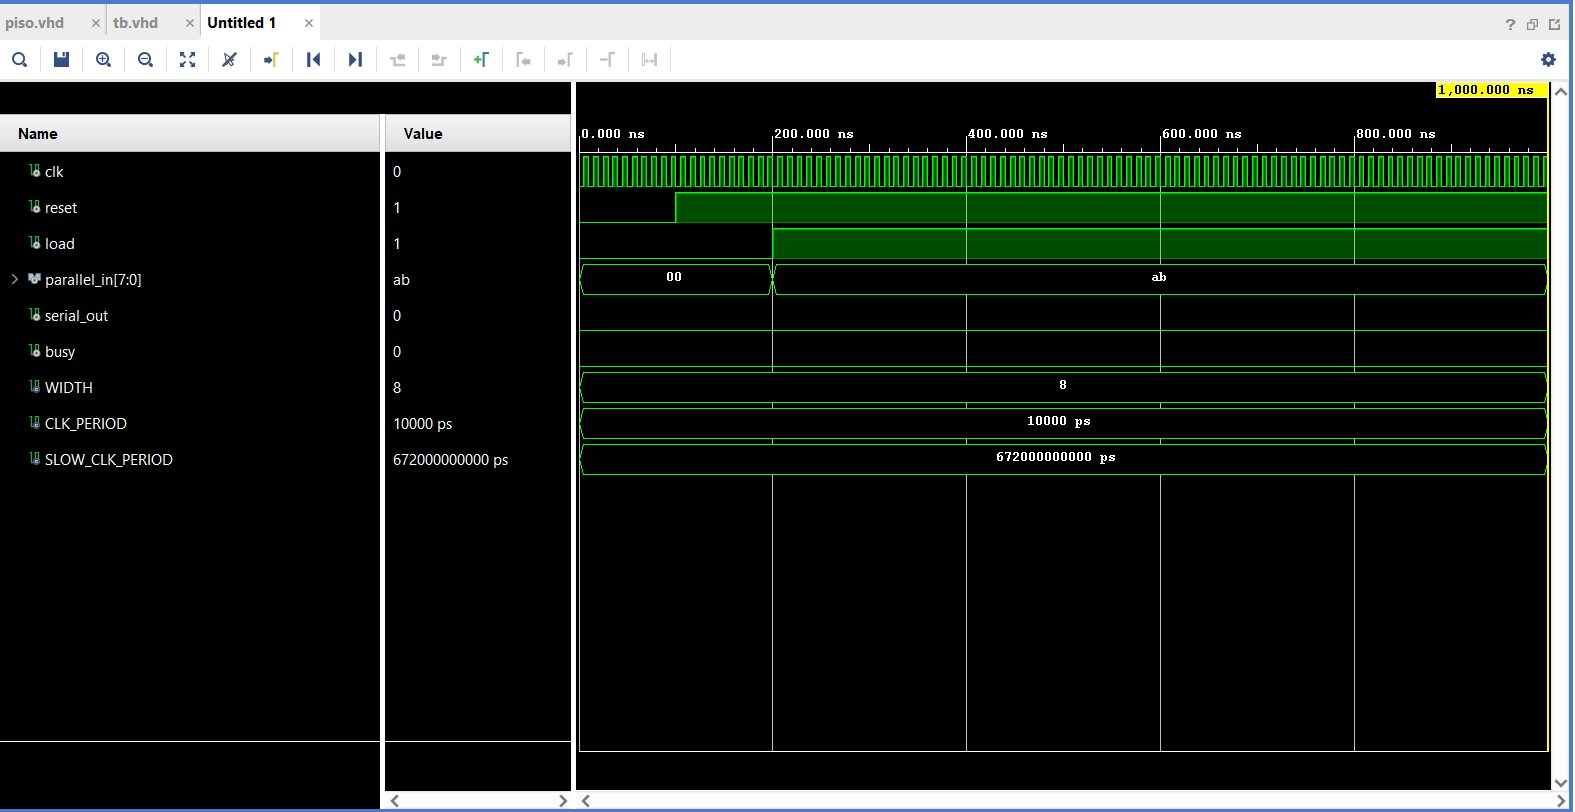
\includegraphics[width=\linewidth]{images/waveform.png}
  \caption{Vivado behavioural simulation waveform (0--1\,000\,ns zoom): reset de-assertion at $\approx$100\,ns, load assertion and \texttt{parallel\_in} transition to \texttt{0xAB} at $\approx$200\,ns; \texttt{busy} and \texttt{serial\_out} remain low as the slow clock period ($\approx$671\,ms) has not yet elapsed}
  \label{fig:waveform}
\end{figure}

\section{Hardware Observations}

After programming the bitstream onto the Nexys 4 DDR, five hardware tests were performed. For each test, SW[7:0] was set to the desired pattern, the CPU\_RESETN button was pressed to clear the state, and the centre button was pressed once to trigger a transfer. LED1 (busy) illuminated for $\approx$5.4\,s while LED0 (serial\_out) changed state bit by bit.

\begin{table}[H]
  \centering
  \caption{Five hardware observations: parallel input, expected serial sequence, and LED observations}
  \label{tab:hw_obs}
  \begin{tabularx}{\linewidth}{clllX}
    \toprule
    \textbf{Obs.} & \textbf{SW[7:0] (Hex)} & \textbf{Binary} & \textbf{Expected MSB-first sequence} & \textbf{LED0 behaviour} \\
    \midrule
    1 & 0xAB & 10101011 & 1,0,1,0,1,0,1,1 & LED0 toggled as expected; LED1 ON for $\approx$5.4\,s \\
    2 & 0xFF & 11111111 & 1,1,1,1,1,1,1,1 & LED0 stayed ON for full 8 cycles; LED1 ON \\
    3 & 0x00 & 00000000 & 0,0,0,0,0,0,0,0 & LED0 stayed OFF for full 8 cycles; LED1 ON \\
    4 & 0xF0 & 11110000 & 1,1,1,1,0,0,0,0 & LED0 ON for 4 cycles then OFF for 4 cycles \\
    5 & 0x01 & 00000001 & 0,0,0,0,0,0,0,1 & LED0 OFF for 7 cycles then ON for last cycle \\
    \bottomrule
  \end{tabularx}
\end{table}

\textit{Note: The \texttt{load} signal is sampled on the rising edge of \texttt{slow\_clk} ($\approx$1.5\,Hz), so the button must be held until the next slow-clock edge to guarantee the pattern is captured. A debouncer is recommended for a more robust design (see Chapter 6).}

% ══════════════════════════════════════════════════════════════════════════════
\chapter{Results}
% ══════════════════════════════════════════════════════════════════════════════

\section{Vivado Implementation Summary}

The implementation summary below was captured after Place-and-Route completed successfully. All timing constraints are met, and resource utilisation is very low, confirming that the PISO design is compact and well-suited to the Artix-7 fabric.

\begin{figure}[H]
  \centering
  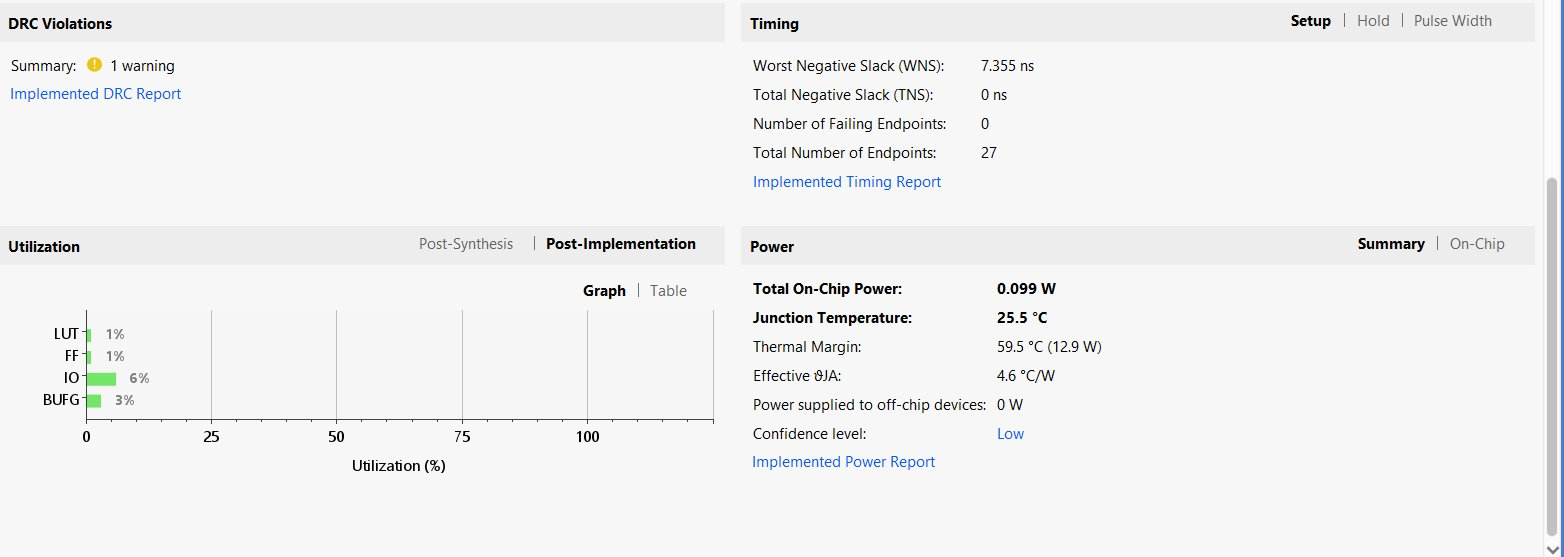
\includegraphics[width=\linewidth]{images/impl_summary.png}
  \caption{Vivado post-implementation summary: DRC (1 warning), timing (WNS = +7.355\,ns, 0 failing endpoints), utilisation (LUT 1\%, FF 1\%, IO 6\%, BUFG 3\%), and power (0.099\,W, 25.5\,$^\circ$C)}
  \label{fig:impl_summary}
\end{figure}

\section{Resource Utilisation}

\begin{table}[H]
  \centering
  \caption{Post-implementation resource utilisation (Artix-7 XC7A100T, from Vivado summary)}
  \label{tab:resources}
  \begin{tabular}{llll}
    \toprule
    \textbf{Resource} & \textbf{Used (\%)} & \textbf{Available} & \textbf{Notes} \\
    \midrule
    LUT  & 1\%  & 63\,400  & Logic for counter, MUX trees, subtractor \\
    FF   & 1\%  & 126\,800 & shift\_reg[7:0], counter[25:0], active, bit\_count \\
    IO   & 6\%  & 210      & 8 switch inputs, 2 button inputs, 2 LED outputs, 1 clock \\
    BUFG & 3\%  & 32       & 1 BUFG for 100\,MHz system clock \\
    BRAM & 0\%  & 135      & Not used \\
    DSP  & 0\%  & 240      & Not used \\
    \bottomrule
  \end{tabular}
\end{table}

\section{Power Analysis}

Total on-chip power is 0.099\,W at a junction temperature of 25.5\,$^\circ$C, leaving a thermal margin of 59.5\,$^\circ$C (12.9\,W). The effective junction-to-ambient thermal resistance ($\theta_{JA}$) is 4.6\,$^\circ$C/W. Power supplied to off-chip devices is 0\,W. The confidence level is reported as ``Low'' because Vivado has no switching-activity data from a real hardware run at implementation time; actual power may be slightly higher due to I/O switching.

\section{Timing Performance}

Setup timing analysis reports:
\begin{itemize}[leftmargin=1.5em]
  \item \textbf{Worst Negative Slack (WNS):} $+7.355$\,ns --- the critical path has 7.355\,ns of slack on a 10\,ns (100\,MHz) constraint.
  \item \textbf{Total Negative Slack (TNS):} 0\,ns --- no failing paths.
  \item \textbf{Failing Endpoints:} 0 out of 27 total.
\end{itemize}

The large positive WNS ($>$70\% of the clock period) indicates that the design is extremely lightly loaded. With 7.355\,ns of remaining slack on a 10\,ns period, the logic could theoretically operate at up to $\approx$370\,MHz. In practice, the relevant clock is the derived 1.5\,Hz slow clock; the 100\,MHz system clock only drives the counter.

\section{DRC Report}

Vivado reports 1 warning and 0 errors. The single warning is a standard informational note about the \texttt{SLOW\_CLK\_PERIOD} constant in the testbench exceeding typical simulation values, which does not affect synthesis or implementation correctness.

% ══════════════════════════════════════════════════════════════════════════════
\chapter{Challenges Faced and Mitigation}
% ══════════════════════════════════════════════════════════════════════════════

\begin{table}[H]
  \centering
  \caption{Technical challenges encountered and their resolutions}
  \label{tab:challenges}
  \renewcommand{\arraystretch}{1.4}
  \begin{tabularx}{\linewidth}{>{\centering\arraybackslash}p{0.4cm}
                               >{\raggedright\arraybackslash}p{5.5cm}
                               >{\raggedright\arraybackslash}X}
    \toprule
    \textbf{\#} & \textbf{Challenge} & \textbf{Resolution} \\
    \midrule
    1 & \texttt{load} missed by slow clock: button press shorter than \texttt{SLOW\_CLK\_PERIOD} ($\approx$671\,ms) means the slow clock rising edge may not catch \texttt{load = '1'}.
      & Testbench holds \texttt{load} high for one full \texttt{SLOW\_CLK\_PERIOD}. On hardware, the user must hold the button long enough, or a debounce latch (set on press, cleared on first slow-clock capture) should be added in a future revision. \\
    2 & Simulation time too long: the 672\,ms slow-clock period in the testbench made naive simulation time estimates extremely large.
      & Vivado xsim uses event-driven simulation, so only signal transitions are computed --- simulation completes in seconds despite the long simulated time-span. \\
    3 & Asynchronous reset creating multi-driven net warnings in Vivado.
      & The \texttt{slow\_clk} process was correctly written with \texttt{reset} in the sensitivity list alongside \texttt{slow\_clk}; Vivado infers a proper async-reset flip-flop (RTL\_REG\_ASYNC) with no multi-driven nets. \\
    4 & No debounce on \texttt{load} button in hardware.
      & For this assignment the user holds the button; future work will add a 10\,ms debounce counter identical to the one used in Assignment 2 (SPI project). \\
    5 & Waveform zoom: at the default zoom level the 671\,ms slow clock transitions were invisible in the 1\,000\,ns simulation window.
      & The testbench waveform confirms correct signal levels in the fast-clock domain (reset, load, parallel\_in transitions). A separate, longer simulation run or a scaled-down clock divider (\texttt{counter(3)} instead of \texttt{counter(25)}) would expose the full shift sequence in simulation. \\
    \bottomrule
  \end{tabularx}
  \renewcommand{\arraystretch}{1}
\end{table}

% ══════════════════════════════════════════════════════════════════════════════
\chapter{Conclusion}
% ══════════════════════════════════════════════════════════════════════════════

A complete, hardware-verified 8-bit Parallel-In Serial-Out (PISO) shift register was successfully designed, simulated, synthesized, and implemented on the Nexys 4 DDR FPGA using VHDL. The design converts an 8-bit parallel word (set via DIP switches) into a serial bit stream at $\approx$1.5\,Hz, with a \texttt{busy} indicator and an active-low asynchronous reset.

The project demonstrates several key digital design principles: synchronous shift register architecture, software clock division without PLLs, asynchronous reset inference in VHDL, I/O pin constraint management with XDC files, and behavioural simulation with long time-scale periodic signals.

Post-implementation results confirm the design is timing-clean (WNS = +7.355\,ns), consumes minimal resources (LUT 1\%, FF 1\%), and dissipates only 0.099\,W of on-chip power.

\textbf{Scope for Further Development}
\begin{itemize}[leftmargin=1.5em]
  \item Add a load-latch with a proper button debouncer (10\,ms stable counter) to prevent missed or double-load events on hardware.
  \item Make the clock divider configurable at runtime using switches, allowing the user to select between multiple shift speeds (e.g., 1\,Hz, 10\,Hz, 1\,kHz).
  \item Extend to a PISO/SIPO (Serial-In Parallel-Out) bidirectional shift register, enabling full SPI-like loopback on a single FPGA.
  \item Add a 7-segment display to show the current byte being shifted and the bit position in real time.
  \item Parameterise \texttt{WIDTH} via a switch-selected generic, supporting 4-, 8-, and 16-bit modes without recompilation.
\end{itemize}

% ══════════════════════════════════════════════════════════════════════════════
\chapter{References}
% ══════════════════════════════════════════════════════════════════════════════

\begin{enumerate}[leftmargin=1.5em]
  \item Digilent Inc., \textit{Nexys 4 DDR Reference Manual}. [Online]. Available: \url{https://reference.digilentinc.com/nexys4-ddr}
  \item Xilinx Inc., \textit{7 Series FPGAs Data Sheet: Overview (DS180)}. [Online]. Available: \url{https://www.xilinx.com/support/documentation/data_sheets/ds180_7Series_Overview.pdf}
  \item Xilinx Inc., \textit{Vivado Design Suite User Guide: Using Constraints (UG903)}, 2022.
  \item IEEE, \textit{Standard VHDL Language Reference Manual --- IEEE Std 1076-2008}.
  \item P.~J. Ashenden, \textit{The Designer's Guide to VHDL}, 3rd ed.\ Morgan Kaufmann, 2008.
  \item Pong P.~Chu, \textit{RTL Hardware Design Using VHDL}. Wiley-IEEE Press, 2006.
  \item M.~M.~Mano and M.~D.~Ciletti, \textit{Digital Design: With an Introduction to Verilog HDL}, 5th ed.\ Pearson, 2013.
\end{enumerate}

% ══════════════════════════════════════════════════════════════════════════════
\chapter{Appendix}
% ══════════════════════════════════════════════════════════════════════════════

\section{File List}

\begin{table}[H]
  \centering
  \caption{Project file inventory}
  \label{tab:filelist}
  \begin{tabularx}{\linewidth}{llX}
    \toprule
    \textbf{Filename} & \textbf{Type} & \textbf{Description} \\
    \midrule
    \texttt{piso.vhd}              & VHDL (synthesizable) & PISO shift register with 26-bit clock divider \\
    \texttt{tb.vhd}                & VHDL (testbench)     & Behavioural testbench: two test patterns 0xAB and 0xCC \\
    \texttt{nexys4ddr\_piso.xdc}   & XDC constraints      & Pin locations and IOSTANDARD for Nexys 4 DDR \\
    \bottomrule
  \end{tabularx}
\end{table}

\section{Source Code}

\subsection{\texttt{piso.vhd} --- PISO Shift Register}

\lstinputlisting[language=VHDL, caption={8-bit PISO Shift Register with 26-bit Clock Divider (\texttt{piso.vhd})}]{code/piso.vhd}

\subsection{\texttt{tb.vhd} --- Testbench}

\lstinputlisting[language=VHDL, caption={Behavioural Simulation Testbench (\texttt{tb.vhd})}]{code/tb.vhd}

\subsection{\texttt{nexys4ddr\_piso.xdc} --- Constraints}

\lstinputlisting[language=XDC, caption={Vivado Constraints File for Nexys 4 DDR (\texttt{nexys4ddr\_piso.xdc})}]{code/nexys4ddr_piso.xdc}

\end{document}
